\chapter{Design}

\section{Overall System Design}

\subsection{Short description of the main parts of the system}

\subsection{System flowcharts showing an overview of the complete system}

\section{User Interface Designs}

\section{Hardwear Spesifiacation}

\section{Program Structure}

\subsection{Top-down design structure charts}

\subsection{Algorithms in pseudo-code for each data transformation process}

\subsection{Object Diagrams}

\subsection{Class Definitions}

\section{Prototyping}

\section{Definition of Data Requirements}

\subsection{Identification of all data input items}

\subsection{Identification of all data output items}

\subsection{Explanation of how data output items are generated}
Blank
\subsection{Data Dictionary}

\begin{tabular}{|p{1.5cm}|p{1.5cm}|l|l|l|p{2.5cm}|}
	\hline
	NAME & DATA TYPE & LENGTH & VALIDATION & EXAMPLE DATA & APPROXIMATE SIZE \\ \hline
	EventID & Integer & 0-9999 & Range & 10 & 4 Bytes \\ \hline
	CourseID & Integer & 0-9999 & Range & 10 & 4 Bytes \\ \hline
	Date & Date & DD/MM/YYYY & Range & 1 & 3 Bytes \\ \hline
	CircuitSeries & Boolean & 0 or 1 & Range & 1 & 2 Bytes \\ \hline
	Handicap10 & Boolean & 0 or 1 & Range & 1 & 2 Bytes \\ \hline
	Handicap25 & Boolean & 0 or 1 & Range & 1 & 2 Bytes \\ \hline
	HillClimb & Boolean & 0 or 1 & Range & 1 & 2 Bytes \\ \hline
	Transmedia & Boolean & 0 or 1 & Range & 1 & 2 Bytes \\ \hline
	Juvenile & Boolean & 0 or 1 & Range & 1 & 2 Bytes \\ \hline
	Code & String & 2 Characters & length & TR & 2 Bytes \\ \hline
	RiderID & Integer & 0-9999 & Range & 10 & 4 Bytes \\ \hline
	Forename & String & 50 Characters & length & Peter & 50 Bytes \\ \hline
	Surname & String & 50 Characters & length & Millard & 50 Bytes \\ \hline
	TCID & Integer & 0-9999 & Range & 10 & 4 Bytes \\ \hline
	Handicap10Points & Integer & 0-350 & Range & 125 & 4 Bytes \\ \hline
	CircuitPoints & Integer & 0-350 & Range & 125 & 4 Bytes \\ \hline
	TransmediaPoints & Integer & 0-350 & Range & 125 & 4 Bytes \\ \hline
	JuvenlePoints & Integer & 0-350 & Range & 125 & 4 Bytes \\ \hline
	CourseID & Integer & 0-9999 & Range & 10 & 4 Bytes \\ \hline
	RecordID & Integer & 0-9999 & Range & 10 & 4 Bytes \\ \hline
	RideTime & Time & HH:MM:SS & Range & 01:25:23 & 3 Bytes \\ \hline
	HandicapTime & Time & HH:MM:SS & Range & 00:25:23 & 3 Bytes \\ \hline
	RacePosition & Integer & 1-50 & Range & 05 & 4 Bytes \\ \hline
	Club & String & 50 Characters & Length & Team Cambridge & 100 Bytes \\ \hline
	Age & Integer & 12 – 99 & Range & 18 & 4 Bytes \\ \hline
\end{tabular}

\subsection{Identification of appropriate storage media}

\section{Database Design}

\subsection{Normalisation}

\subsubsection{ER Diagrams}
\begin{figure}[H]
    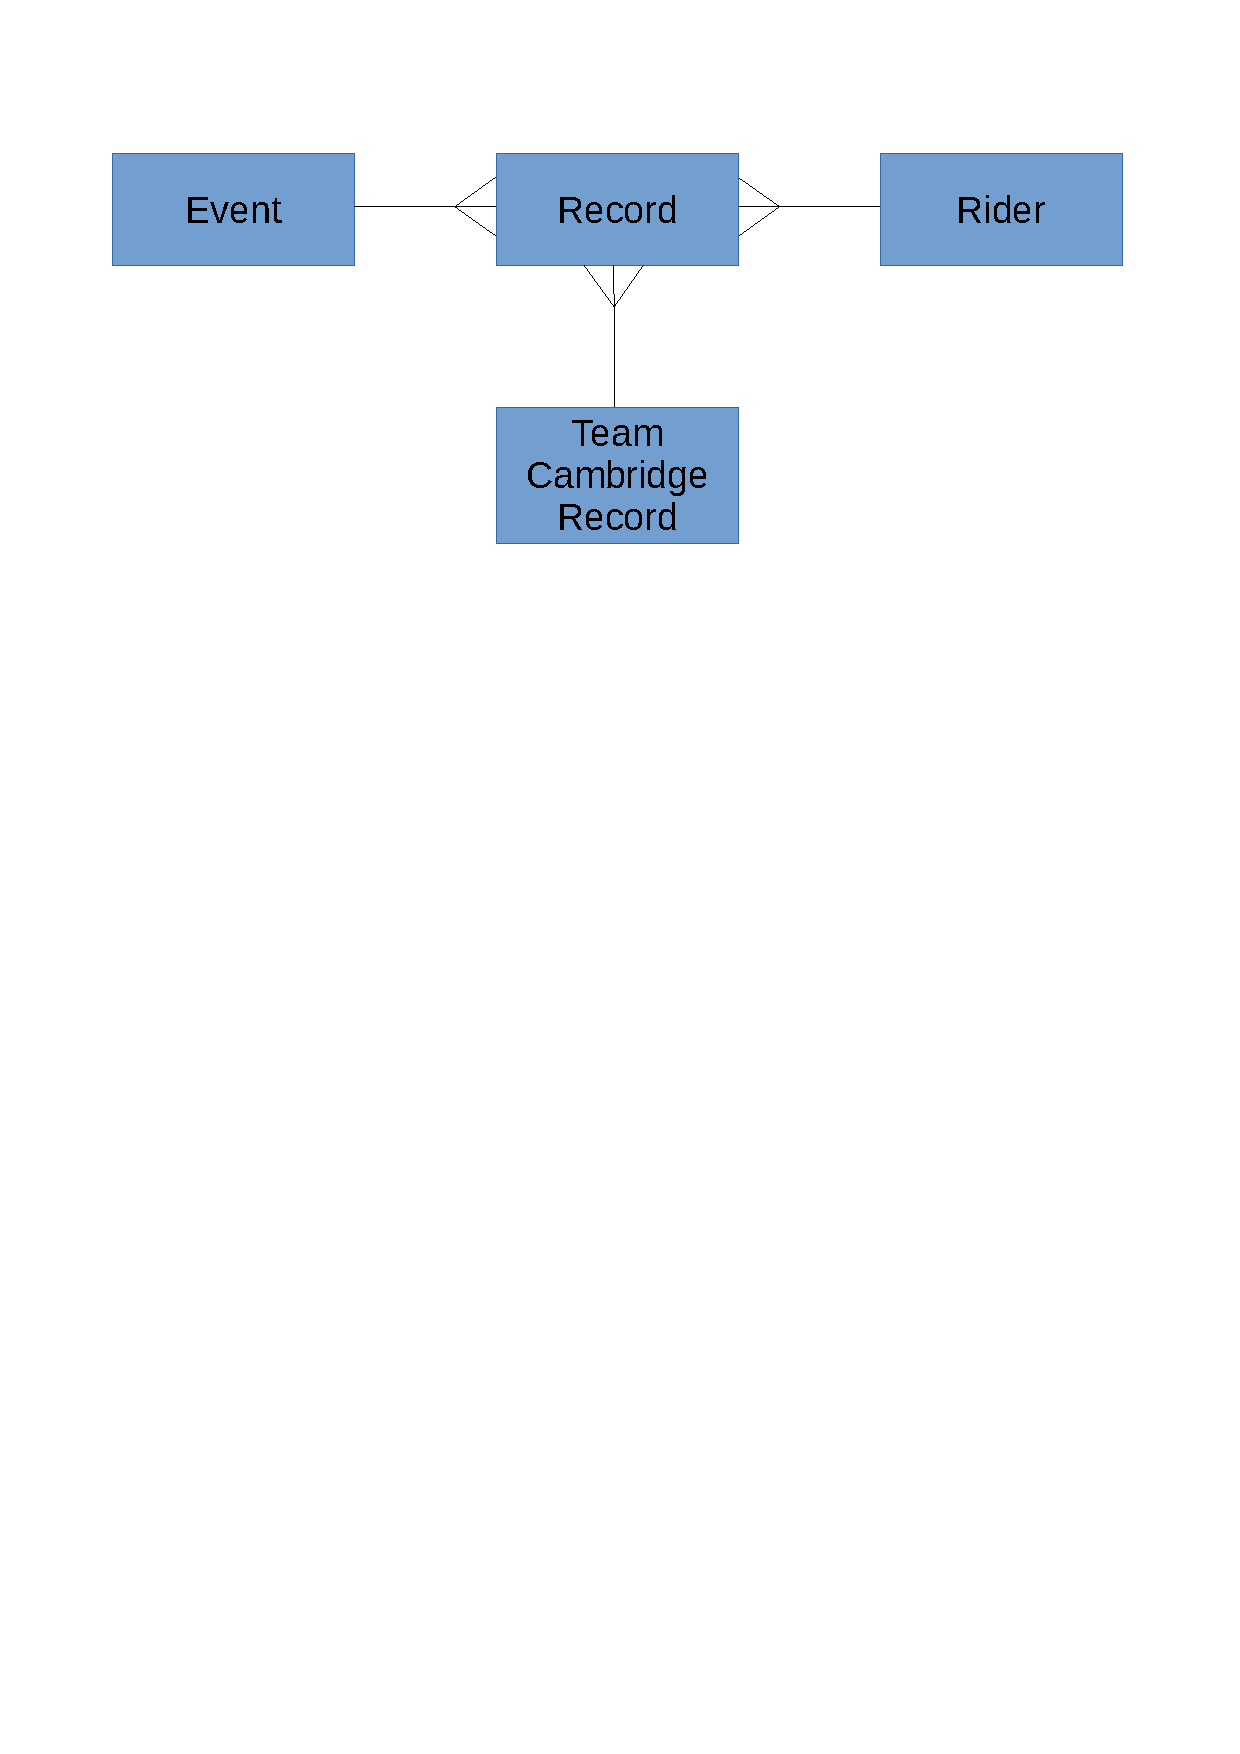
\includegraphics[width=\textwidth]{./ER/ERDesing.pdf}
\end{figure}

\subsubsection{Entity Descriptions}

Rider(\underline{RiderID}, Forename, Surname)

Event(\underline{EventID}, \emph{CourseID} , \emph{EventTypeID}, Date )

Team Cambride Record(\underline{TCID}, \emph{RiderID}, \emph{EventID}, Handicap10Points, CircuitPoints, TransmediaPoints, JuvenilePoints)

Record(\underline{RecordID}, \emph{RiderID}, \emph{EventID}, RdieTime, Age)

Club(\underline{ClubReferance}, \emph{RiderID}, Club, DateJoined, DateLeft)

Course(\underline{CourseID}, CourseCode, CourseDistance)

EventType(\underline{EventTypeID}, EventPrimaryType, EventSecondaryType, EventTertiaryType)

\subsubsection{UNF to 3NF}
\underline{UNF}


\begin{tabular}{l l l}
EventID       & Age              & Date               \\
EventTypeID   & EventPrimaryType & EventSecondaryType \\
ClubReferance & RiderID          & Forename           \\
Surname       & TCID             & EventPoints        \\
Club          & RecordID         & RideTime           \\
CourceID      & CourceCode       & CourceDistance     \\
DateJoined    & DateLeft         & EventTertiaryType  \\
\end{tabular}

\underline{1NF}

\begin{tabular}{|l|l|}
\hline
REPEATING            & NON-REPEATING       \\ \hline
\underline{RecordID} & \underline{EventID} \\ \hline
\underline{EventID}  & Date                \\ \hline
TCID                 & CourseID            \\ \hline
EventPoints          & CourseCode          \\ \hline
EventTypeID          & CorseDistance       \\ \hline 
EventSubType         &                     \\ \hline 
RideTime             &                     \\ \hline 
Age                  &                     \\ \hline
RiderID              &                     \\ \hline
Forename             &                     \\ \hline
Surname              &                     \\ \hline
ClubReferance        &                     \\ \hline
Club                 &                     \\ \hline
DateJoined           &                     \\ \hline
DateLeft             &                     \\ \hline
\end{tabular}




\underline{2NF}

\begin{tabular}{|l|l|}
\hline
\underline{RiderID} & \underline{EventID} \\ \hline
Forename            & Date                \\ \hline
Surname             & CourceID            \\ \hline
ClubReferance       & CourceCode          \\ \hline
Club                & CourceDistance      \\ \hline
DateJoined          &                     \\ \hline
DateLeft            &                     \\ \hline
                    &                     \\ \hline
\underline{RiderID} &                     \\ \hline
\underline{EventID} &                     \\ \hline 
TCID                &                     \\ \hline 
EventPoints         &                     \\ \hline
RecordID            &                     \\ \hline
RideTime            &                     \\ \hline
HandicapTime        &                     \\ \hline
RacePosition        &                     \\ \hline
Age                 &                     \\ \hline
EventTypeID         &                     \\ \hline
EventSubType        &                     \\ \hline
\end{tabular}

\underline{3NF}

\begin{tabular}{|l|l|l|l|}
\hline
\begin{tabular}{l}
	\underline{RiderID}  \\
	Forename             \\
	Surname              \\
\end{tabular} & \begin{tabular}{l}
	\underline{EventID}  \\
	\emph{CourseID }     \\
	\emph{EvetnTypeID}    \\
	Date                 \\
\end{tabular} & \begin{tabular}{l}
	\\
	\underline{TCID}     \\
	\emph{RiderID}       \\
	\emph{EventID}       \\
	Handicap10Points     \\
	CircuitPoints        \\
	TransmediaPoints     \\
	JuvenilePoints       \\
	\\
\end{tabular} & \begin{tabular}{l}
	\underline{RecordID} \\
	\emph{RiderID}       \\
	\emph{EventID}       \\
	RideTime             \\
	Age                  \\
\end{tabular} \\ \hline
\begin{tabular}{l}
	\\
	\underline{ClubReferance} \\
	\emph{RiderID}            \\
	Club                      \\
	DateJoined                \\
	DateLeft                  \\
	\\
\end{tabular} & \begin{tabular}{l}
	\underline{CourseID} \\
	CourseCode           \\
	CourseDistance       \\
\end{tabular} & \begin{tabular}{l}
	\underline{EvntTypeID} \\
	EventPrimaryType       \\
	EventSecondaryType     \\
	EventTertiaryType      \\
\end{tabular} & \\
\hline
\end{tabular}

\section{Security and Integrity of the System and Data}

\subsection{Security and Integrity of Data}

\subsection{System Security}

\section{Validation}

\section{Testing}

\begin{landscape}
\subsection{Outline Plan}

\begin{center}
    \begin{tabular}{|p{2cm}|p{5cm}|p{5cm}|p{4cm}|}
        \hline
        \textbf{Test Series} & \textbf{Purpose of Test Series} & \textbf{Testing Strategy} & \textbf{Strategy Rationale}\\ \hline
        Example & Example & Example & Example \\ \hline
    \end{tabular}
\end{center}

\subsection{Detailed Plan}

\begin{center}
    \begin{longtable}{|p{1.5cm}|p{2.5cm}|p{2.5cm}|p{2cm}|p{2cm}|p{2cm}|p{2cm}|p{2cm}|}
        \hline
        \textbf{Test Series} & \textbf{Purpose of Test} & \textbf{Test Description} & \textbf{Test Data} & \textbf{Test Data Type (Normal/ Erroneous/ Boundary)} & \textbf{Expected Result} & \textbf{Actual Result} & \textbf{Evidence}\\ \hline
        Example & Example & Example & Example & Example & Example & Example & Example \\ \hline
    \end{longtable}
\end{center}
\end{landscape}
